\documentclass[a4paper]{article}

\usepackage[slovene]{babel}
\usepackage[utf8x]{inputenc}
\usepackage{amsmath}
\usepackage{graphicx}
\usepackage{listings} % Required for insertion of code
\usepackage{courier} % Required for the courier font
\usepackage{color}
\usepackage{listings}
\usepackage{setspace}

\definecolor{Code}{rgb}{0,0,0}
\definecolor{Decorators}{rgb}{0.5,0.5,0.5}
\definecolor{Numbers}{rgb}{0.5,0,0}
\definecolor{MatchingBrackets}{rgb}{0.25,0.5,0.5}
\definecolor{Keywords}{rgb}{0,0,1}
\definecolor{self}{rgb}{0,0,0}
\definecolor{Strings}{rgb}{0,0.63,0}
\definecolor{Comments}{rgb}{0,0.63,1}
\definecolor{Backquotes}{rgb}{0,0,0}
\definecolor{Classname}{rgb}{0,0,0}
\definecolor{FunctionName}{rgb}{0,0,0}
\definecolor{Operators}{rgb}{0,0,0}
\definecolor{Background}{rgb}{1,1,1}

\lstnewenvironment{python}[1][]{
\lstset{
%numbers=left,
%numberstyle=\footnotesize,
%numbersep=1em,
xleftmargin=1.5em,
framexleftmargin=1em,
framextopmargin=1em,
framexbottommargin=1em,
showspaces=false,
showtabs=false,
showstringspaces=false,
frame=l t b u r,
tabsize=4,
% Basic
basicstyle=\ttfamily\small\setstretch{1},
backgroundcolor=\color{Background},
language=Python,
% Comments
commentstyle=\color{Comments}\slshape,
% Strings
stringstyle=\color{Strings},
morecomment=[s][\color{Strings}]{"""}{"""},
morecomment=[s][\color{Strings}]{'''}{'''},
% keywords
morekeywords={import,from,class,def,for,while,if,is,in,elif,else,not,and,or,print,break,continue,return,True,False,None,access,as,,del,except,exec,finally,global,import,lambda,pass,print,raise,try,assert},
keywordstyle={\color{Keywords}\bfseries},
% additional keywords
morekeywords={[2]@invariant},
keywordstyle={[2]\color{Decorators}\slshape},
emph={self},
emphstyle={\color{self}\slshape},
%
}}{}

\title{Poročilo seminarske naloge}
\author{Simon Ivanšek, Andraž Vrhovec}

\begin{document}
\maketitle

\section{Uvod}
Tema seminarske naloge je spodbujevano učenje. Pri spodbujevanem učenju imamo agenta, ki izvaja akcije v okolju, od okolja pa dobi nagrado, novo stanje in možne akcije iz tega stanja. Za seminarsko nalogo smo morali implementirati tako agenta kot okolje. Za implementacijo agenta je vsaka skupina dobila natančno določen algoritem, okolje smo si pa lahko zamislili sami. 

Naša skupina je morala za agenta implementirati "Active ADP with policy iteration" algoritem, za okolje pa smo si izbrali igro Brick Breaker. 

\section{Agent}
Pri spodbujevanem učenju je naloga agenta, da se nauči zaporedja izvajanja akcij v okolju. Takemu zaporedju akcij pravimo načrt (ang. policy).  Agent to počne tako, da se premika iz stanja v nova stanja z akcijami, ki so dovoljene v novem stanju in za to dobiva nagrado. Naš agent na začetku o okolju ne ve ničesar. Ne pozna stanj, akcij, funkcije verjetnosti prehodov med stanji \(P(s' | s, a)\), niti funkcije nagrad \(R(s)\). Vse kar ve o okolju sta začetno stanje in možne akcije iz začetnega stanja. Skozi iteracije se potem agent vsega tega nauči tako, da na začetku zgradi naključni načrt, ki ga izboljšuje z računanjem pričakovane koristnosti (ang. expected utility) vsake akcije po naslednji enačbi:

\[\sum_{a} P(s' | s, a) u(s')\]

Akcija, ki ima največjo koristnost se zamenja z naključno izbrano akcijo. Poleg računanja koristnosti vsake akcije, agent še izračuna koristnost za vsako stanje v katerem je bil glede na funkcijo verjetnosti prehodov \(P(s' | s, a)\),  ki služi za kasnejše iteracije. Koristnost stanj izračuna po naslednji enačbi:

\[\gamma * \sum_{s'} P(s' | s, a) u(s')\ \]
Na ta način si agent iterativno gradi model sveta, funkcijo \(P(s'| s, a)\) in funkcijo \(R(s)\). 

Cilj agenta je, da se nauči takega zaporedja izvajanja akcij, ki mu prinese največjo končno nagrado. Pri iskanju optimalnega načrta naš agent uporablja Bellmanovo enačbo, kjer je \(U^{\pi}(s)\) optimalni načrt:

\[ U^{\pi} (s) = R(s) + \gamma \sum_{s'} P(s' | s, a)  U^\pi (s') \]

\subsection{Raziskovanje ali izkoriščanje}
Agent lahko vedno upošteva samo do sedaj naučeno znanje. Tak agent se nikoli ne nauči ničesar novega, ampak vedno izkorišča le do sedaj naučeno znanje. V determinističnih okoljih je to lahko dobro, v nedeterminističnih pa se ponavadi izkaže za slabo. Zaradi tega smo v našega agenta implementirali tudi funkcijo raziskovanja:

\[ f(u, n) = \left\{
	\begin{array}{l l}
		R^+ & \quad \text{if $n$} < N_e\\
		u & \quad \text{drugače}
	\end{array}
\right.\]

Psevdo koda za našega agenta je prikazana v razdelku 

\section{Okolje}
Za okolje smo si izbrali igro Brick breaker. Gre za igro kjer je na spodnjem delu zaslona ploščica, na zgornjem delu zaslona opeke, vmes pa je žogica, ki se odbija. Naša naloga je, da premikamo ploščico levo in desno tako, da žogica razbije čimveč opek naenkrat (Slika 1). Igro zmagamo, ko razbijemo vse opeke, ali izgubimo če se žogica ne odbije od ploščice ampak "pade na tla". 

\subsection{Stanja in akcije}
Okolje igre Brick breaker je v splošnem nedeterministično in kompleksno, zato smo ga zelo poenostavili. Pri običajni igri Brick breaker je lahko v času \textit{T} ploščica na katerikoli poziciji. Vsako stanje je predstavljeno kot tri-terica:

\[
	(x_{pad}, v_x > 0, bricks)
\]

kjer je $x_{pad}$ pozicija ploščice, $v_x$ x-komponenta hitrosti žogice ($v_x>0$ indicira samo smer, drugače število stanj zelo hitro zraste) in $bricks$ bitni vektor, ki indicira katere opeke so že razbite.
V vsakem stanju se agent odloči za eno od akcij ki so predstavljene kot pari:

\[
(x_{pad}, d)
\]

kjer je $x_{pad}$ nova pozicija ploščice in $d \in \{<, >, .\}$ korekcija smeri žogice. 


Pozicija žogice je predstavljena s seznamom:
\[
(x, y, v_x, v_y)
\]
kjer sta $x$ in $y$ koordinati po x-osi in y-osi, $v_x$ in $v_y$ pa hitrost žogice po x-osi in y-osi. Hitrost žogice po x-osi povečamo ali zmanjšamo za \emph{0.4} glede na izbrano akcijo.

\subsection{Nagrade}

Nagrade agentu povedo kako uspešna je bila neka akcija v določenem stanju. Nagrada je edina uporabna povratna informacija, ki jo agent dobi od okolja. Nagrade morajo biti dobro postavljene, da agenta čimhitreje in po najkrajši privedejo do cilja. 

Nagrade smo definirali za razbitje opeke, za zmago, za poraz in majhno negativno nagrado za vsako akcijo. Nagrade so prikazane v spodnji tabeli:

\begin{center}
\begin{tabular}{|c|c|}
	\hline
	vsaka akcija & -0.1 \\\hline
	razbitje opeke & 0.1 \\\hline
	zmaga & 10 \\\hline
	poraz & -10 \\
	\hline
\end{tabular}
\end{center}

\begin{figure}
\centering
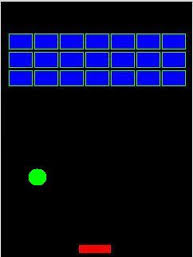
\includegraphics[width=0.5\textwidth]{brick.jpg}
\caption{Brick breaker igra}
\end{figure}

\section{Rezultati}

Zaradi narave okolja 

\begin{table}[h!]
  \begin{tabular}{|c|c|c|c|c|}
  \hline
  Iteracij & $\gamma$ & Najbolsa Nagrada & Najslabsa nagrada & Povprecna nagrada \\\hline
  30         & 0,1   & 10          & -10,4        & 9,9196         \\
  30         & 0,3   & 10          & -10,3        & 9,9798         \\
  30         & 0,5   & 10          & -10,1        & 0,3777         \\
  30         & 0,9   & 10          & -10,1        & -0,05          \\\hline
  50         & 0,1   & 9,9         & -10,1        & 9,8            \\
  50         & 0,3   & 10          & 10           & 10             \\
  50         & 0,5   & 10          & -10,1        & -0,07          \\
  50         & 0,9   & 10          & -10,3        & 0,8216        \\\hline
  \end{tabular}
  \caption{Rezultati}
\end{table}
\begin{figure}[h!]
  \centering
  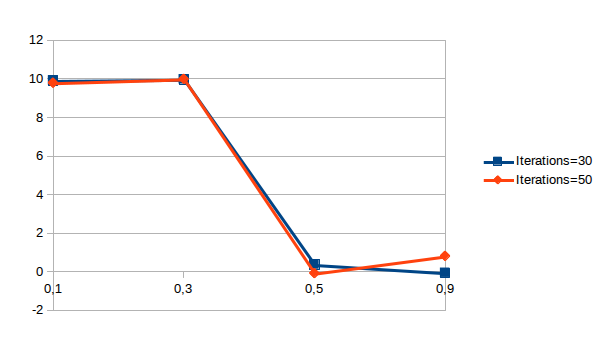
\includegraphics[width=1.0\textwidth]{graf.png}
  \caption{Povprecna nagrada v odvisnosti od parametra $\gamma$}
\end{figure}



\section{Dodatek A}
\begin{figure}[htb]
\begin{python}
def ADPAgent(env):
	model = Model()
	P = None
	lastAction = None
	state = env.getStartingState()
	lastAction = random.choice(env.getActions(state))
	terminal = False

	while terminal is False:
		action = lastAction
		newState, reward, terminal = env.do(state, action)
		percept = (state, action, newState, reward, terminal)
		model.update(percept)
		P = policyIteration(model, env)
		lastAction = performanceElement(newState)
		state = newState
\end{python}
\caption{Psevdo koda v Pythonu za ADP agenta}
\end{figure}

\begin{figure}[htb]
\begin{python}
def policyIteration(model, env):
    U = zeroUtilities(model)
    P = buildRandomPolicy(model)	
   
    converged = False
    while converged is False:
        converged = True
        U = valueDetermination(P, U, model)
        for s in P.keys():
            a = getBestAction(env, model, U, s)
            if a != P.get(s):
                P[s] = a
                converged = False
    return P
\end{python}
\caption{Psevdo koda v Pythonu za policy iteration}
\end{figure}

\begin{figure}[htb]
\begin{python}
def valueDetermination(P, U, model, k = 10):
    R = lambda s: model.avgReward(state) or 0
    maxU = 0

    for i in xrange(k):
        for state in P.keys():
            if model.visits(state) > Ne:
                s = prob * U[newState] for newState, prob in 
                    model.getTransitions(state, P.get(state))
                est = gamma * sum()
            else:
                est = Rplus

            u = R(state) + est
            maxU = max(maxU, u)
            U[state] = u
        
            if maxU >= Rplus:
                Rplus = maxU+1
        return U
\end{python}
\caption{Psevdo koda v Pythonu za racunanje koristnosti stanj}
\end{figure}

\end{document}